\hsection{History}%
\label{sec:history}%
\FloatBarrier%
%
\begin{figure}%
\centering%
%
\subfloat[][%
Sumerian school exercise tablet, Cuneiform tablet no.~10. Between 2200 and 1900~\acrshort{BCE} \href{https://www.loc.gov/item/2020741379}{LCCN2020741379}.%
\label{fig:tablet01}%
]{\tightbox{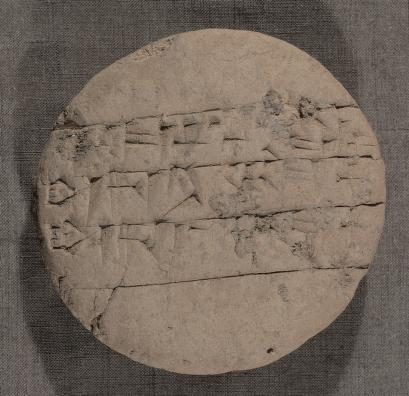
\includegraphics[width=0.17\linewidth]{\currentDir/tablet01}}}%
%
\floatSep%
%
\subfloat[][%
Old Babylonian (Akkadian) ledger of fish, Cuneiform tablet no.~20. Between 2200 and 1900~\acrshort{BCE} \href{https://www.loc.gov/item/2020741389}{LCCN2020741389}.%
\label{fig:tablet02}%
]{\tightbox{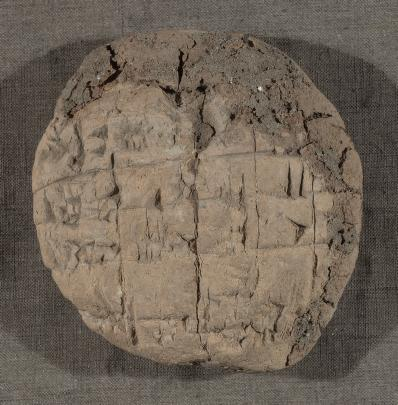
\includegraphics[width=0.17\linewidth]{\currentDir/tablet02}}}%
%
\floatSep%
%
\subfloat[][%
Sumerian cone inscription, Cuneiform tablet no.~22. Between 2200 and 1900~\acrshort{BCE} \href{https://www.loc.gov/item/2020741391}{LCCN2020741391}.%
\label{fig:tablet03}%
]{\tightbox{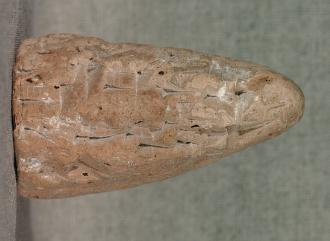
\includegraphics[height=0.17\linewidth,angle=90]{\currentDir/tablet03}}}%
%
\floatSep%
%
\subfloat[][%
Sumerian bill of sale, Cuneiform tablet no.~23. 2038~\acrshort{BCE} \href{https://www.loc.gov/item/2020741392}{LCCN2020741392}.%
\label{fig:tablet04}%
]{\tightbox{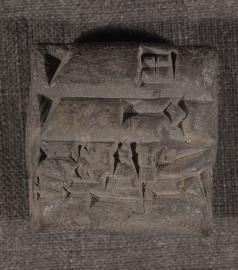
\includegraphics[height=0.17\linewidth]{\currentDir/tablet04}}}%
%
\floatSep%
%
\subfloat[][%
Sumerian votive plaque, Cuneiform tablet no.~25. Between 2144 and 2124~\acrshort{BCE} \href{https://www.loc.gov/item/2020741394}{LCCN2020741394}.%
\label{fig:tablet05}%
]{\tightbox{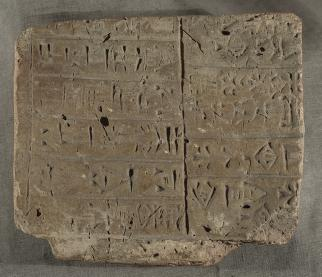
\includegraphics[height=0.17\linewidth,angle=90]{\currentDir/tablet05}}}%
%
\caption{Several clay tablets dating back as far as 2200~\pgls{BCE} from the collection \citetitle{LOCCTFTROGOLTSI}~\cite{LOCCTFTROGOLTSI}.}%
\label{fig:LOCCTFTROGOLTSI}%
\end{figure}%
%
We will now take a brief look at the history of \pglspl{db}~\cite{S2024D:THOD,Q2022ATODHDM,M2024ABHOD,YM2024DDMSD,F2021ABHODM}.
By understanding the history of \pglspl{dbms}, we can better understand the current behavior and features of \pglspl{db}.

People began storing and processing information a very long time ago.
A driving force to collect and analyze data must have been the management of limited resources.
Some of the earliest discovered writings are Sumerian accounting and tax records on clay tablets from Mesopotamia, dating back four thousand years~\cite{LOCCTFTROGOLTSI,T1999CTRAA,KT2021IAITWWICF4Y}, as illustrated in \cref{fig:LOCCTFTROGOLTSI}.
The collection and analysis of information never stopped from then onwards.

\begin{figure}%
\centering%
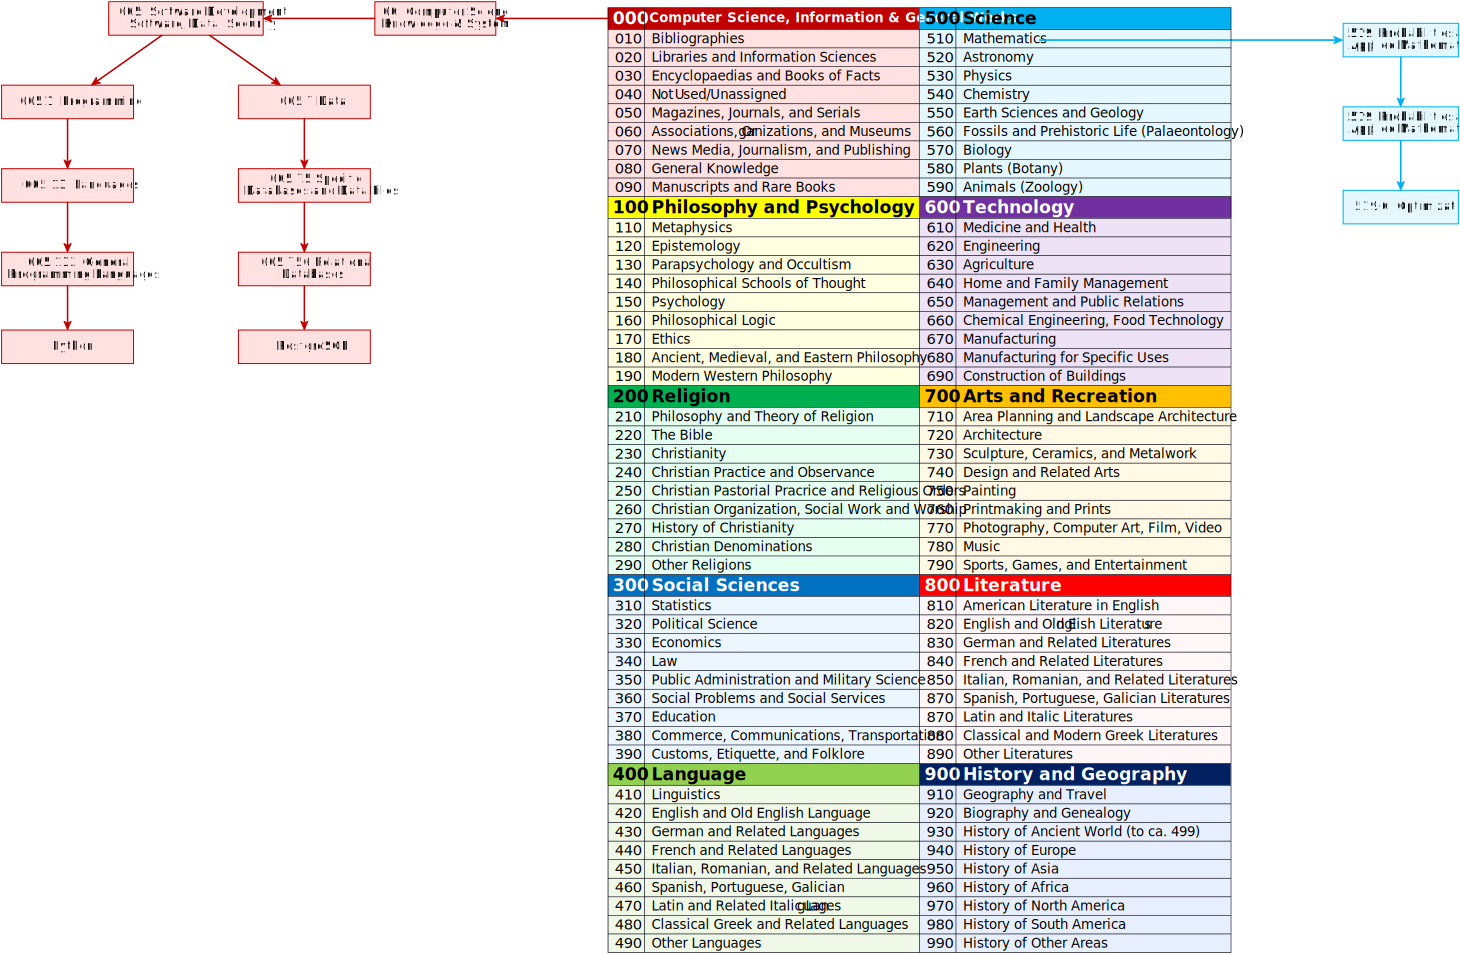
\includegraphics[width=0.9\linewidth]{\currentDir/mds}%
\caption{An illustration of the Melvil Decimal System~\cite{L2025MMDS}, a free variant of the Dewey Decimal System named after its inventor Melvil Dewey, and the steps needed to locate books on \python, \postgresql, or optimization.}%
\label{fig:mds}%
\end{figure}%
%
\begin{figure}%
\centering%
%
\subfloat[][Sketches of \citeauthor{H1892MFTS}'s tabulator machine that used punched bards from his \citeyear{H1892MFTS} patent~\cite{H1892MFTS}.%
\label{fig:H1892MFTS}]{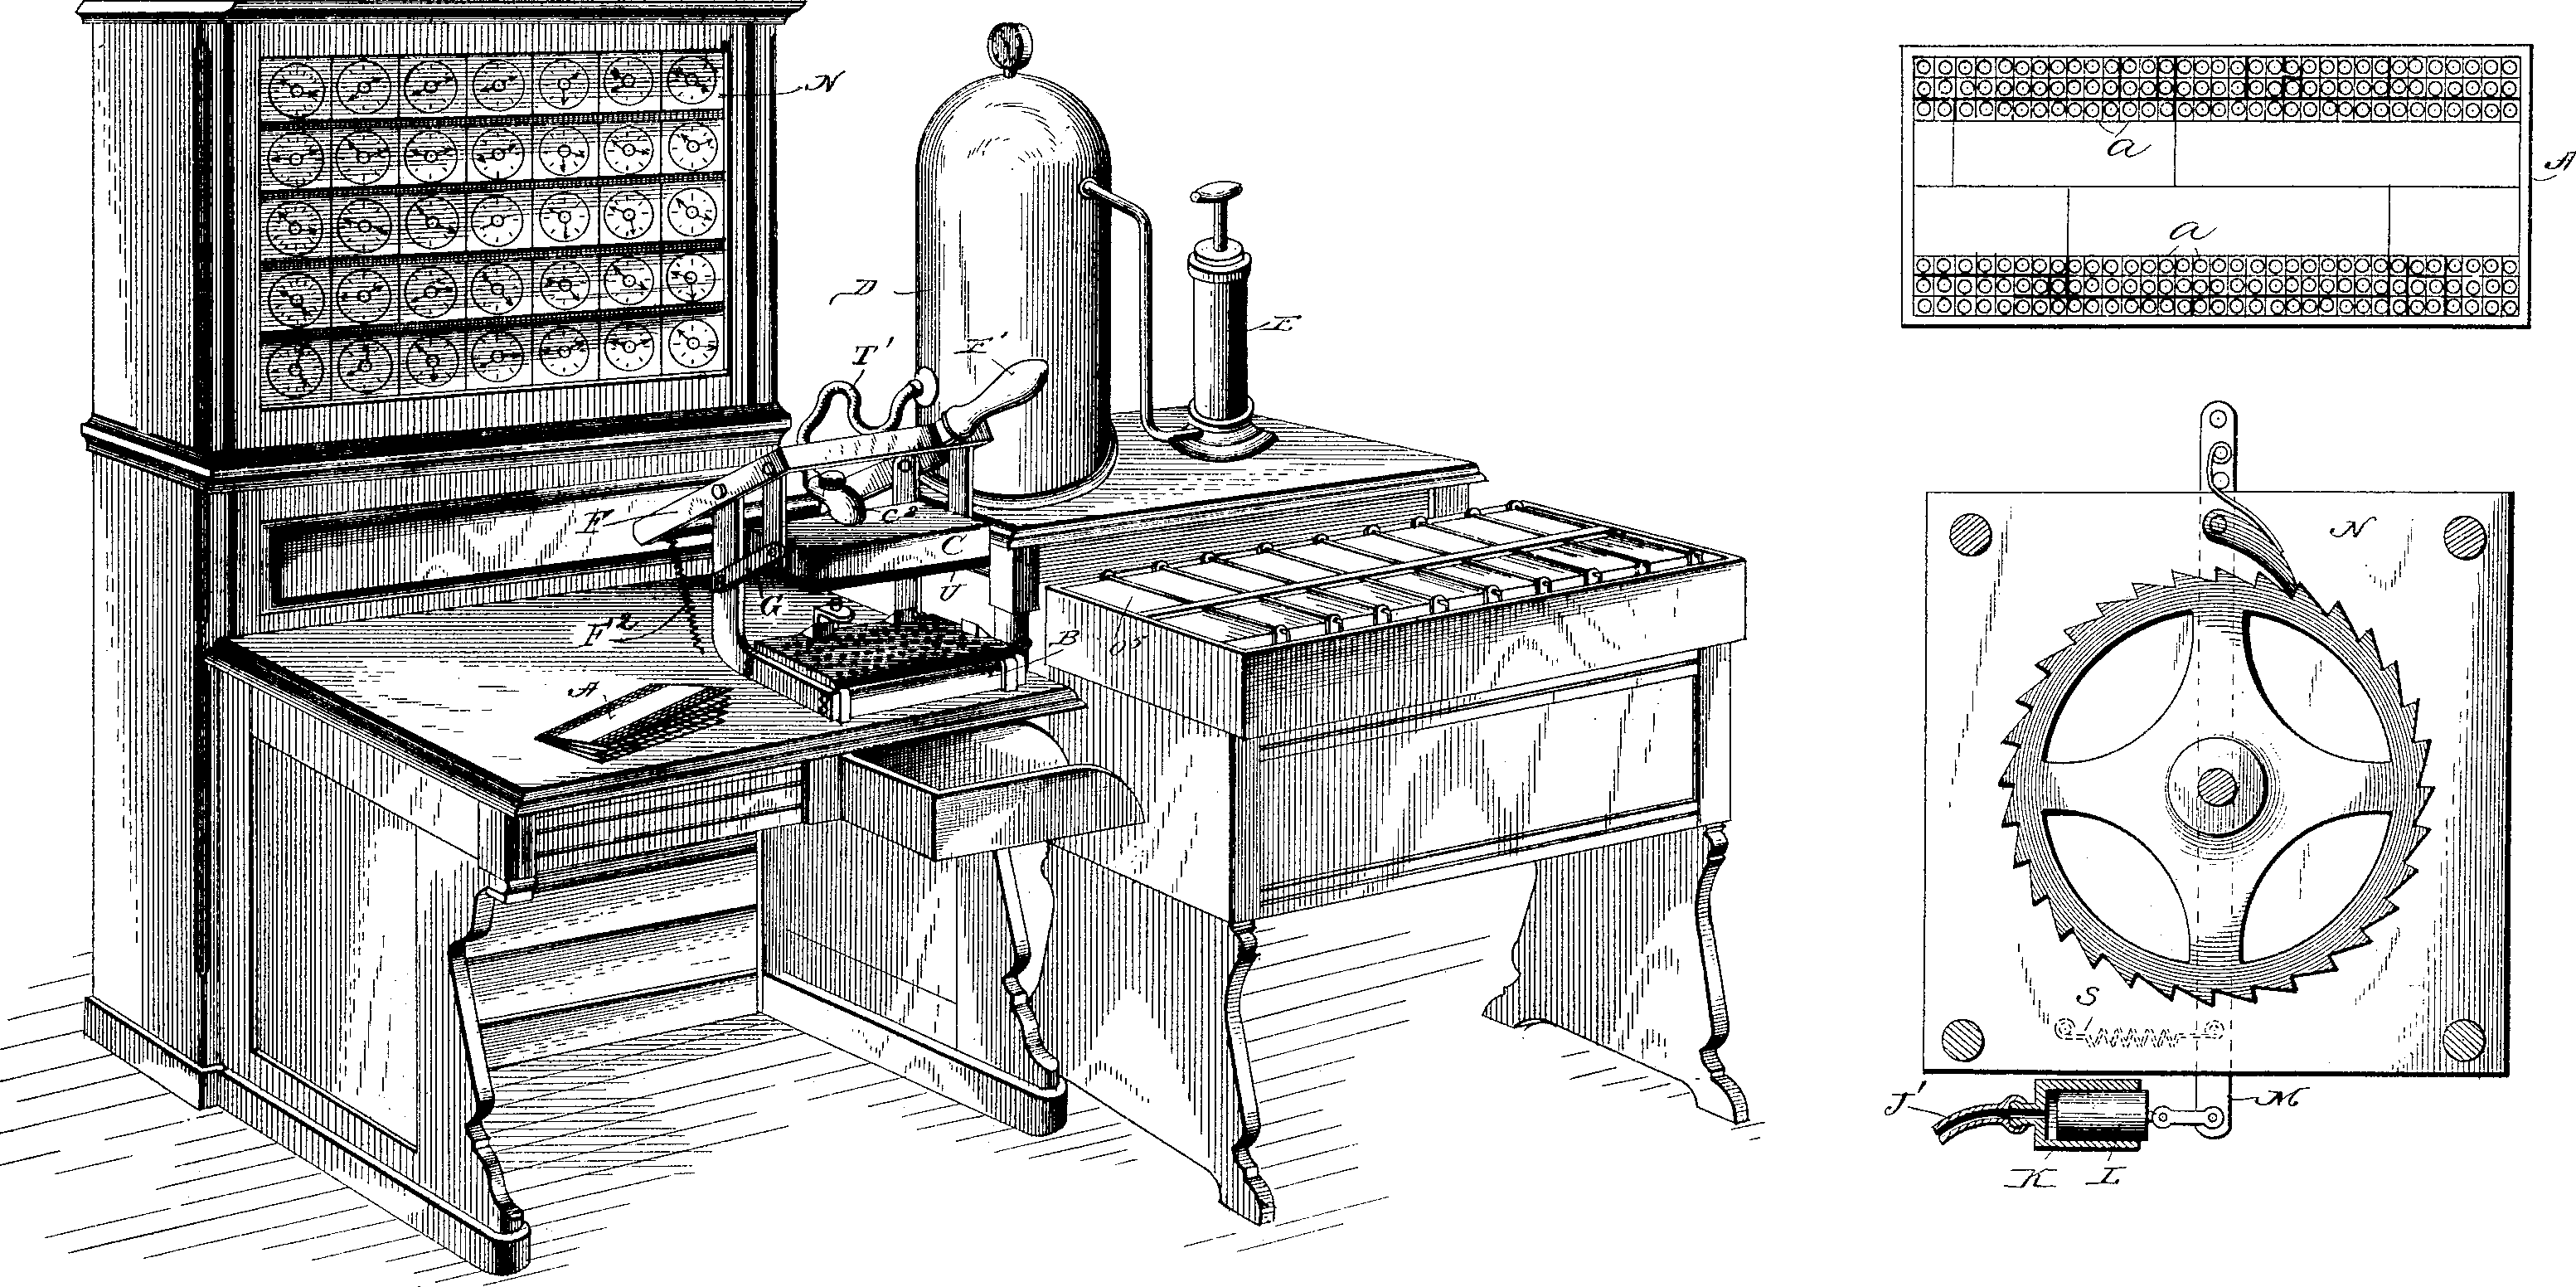
\includegraphics[width=0.62\linewidth]{\currentDir/hollerithMachine}}%
%
\floatSep%
%
\subfloat[][An IBM 029 punched card. %
Source:~\cite{T2018TI0CP}, licensed under \href{https://creativecommons.org/licenses/by-sa/4.0/}{CC~BY\nobreakdashes-SA~4.0}.%
\label{fig:T2018TI0CP}]{%
\parbox[t]{0.35\linewidth}{\centering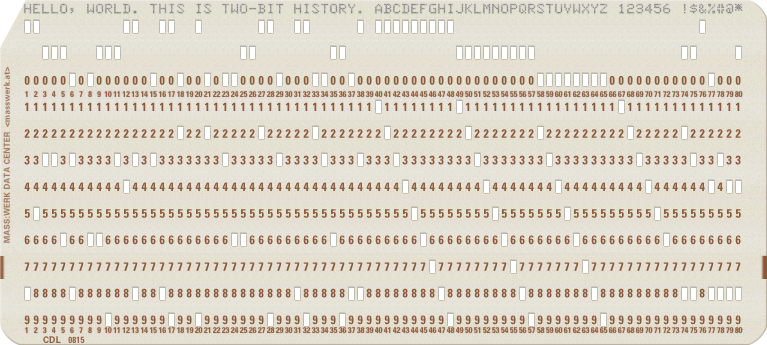
\includegraphics[angle=90,height=0.999\linewidth]{\currentDir/ibm029punchedCard}}%
}%
%
\caption{A very early patented machine using punched cards and an IBM 029 punched card, which was available in the 1960s to 1980s.}%
\end{figure}%

When much data is stored, three big questions emerge:
\emph{How do we store the information?},
\emph{How can I find a specific record?},
and
\emph{How can we condense and extract representative information from all of this data?}

Examples for the data organization include the Dewey Decimal Classification system for organizing books in a libray, which emerged in the 1870s~\cite{CM2003DDCPAA,OCLC2019ITTDDC}.
This system and similar systems as the one illustrated in \cref{fig:mds} are still in use today.
Not much later, we enter the earliest stage of data processing with machines.
Data storage happened by using physical tools~\cite{H1997SATAPCS1}.
The punched cards system by \citeauthor{H1884AFCS}, patented in the late 1880s~\cite{H1884AFCS,H1892MFTS}, was used in the 1890s US~Census.
The automatic processing of these cards allowed the census to finish under budget and ahead of time~\cite{ITIPCTPORTTIAOHMOTWD}.
\citeauthor{H1884AFCS}'s Tabulating Machine Company eventually merged with three other companies into International Business Machines~(IBM).
Punch cards similar to the latter model shown in \cref{fig:T2018TI0CP} made up 20\% of the revenue of IBM as late as the mid\nobreakdashes-1950s~\cite{ITIPCTPORTTIAOHMOTWD}.

In addition to punch cards, reels of punched tape emerged as data storages and later magnetic tapes.
The way data can be retrieved depends on how the data is stored.
Punch cards can be sorted, stacked, and otherwise cleverly be arranged to access information quickly.
Tape-based storages requires us to sequentially spool through the tape to find the data we are looking for.
Either way, efficient organization of data and media became more and more important.
In \citeyear{BIF1958OARORGIALSEP}, the Electronic Recording Machine Accounting~(ERMA) Mark~1 was developed as automated system for organizing banking records~\cite{BIF1958OARORGIALSEP}.
It had features of file system, although the term \inQuotes{files} was meant literally -- they organized paper-based documents, using a structure reminiscent of the aforementioned hierarchical, number-based Dewey categorization method.

\begin{figure}%
\centering%
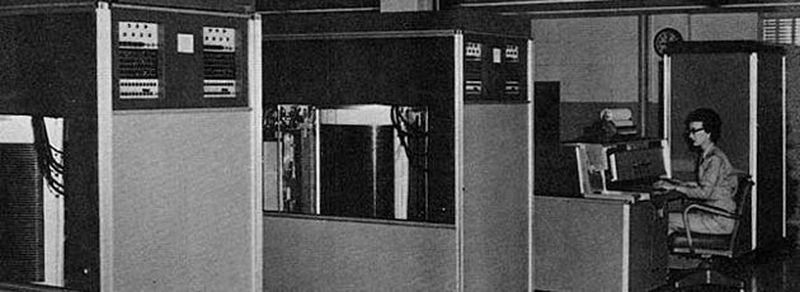
\includegraphics[width=0.7\linewidth]{\currentDir/ramac}%
\caption{Image from 1956:~An IBM 305 RAMAC (right) with two of the (at that time) very new IBM 350 hard disks (middle and left). %
Source:~\cite{G2016I3EKMUDDFW6}.}%
\label{fig:G2016I3EKMUDDFW6}%
\end{figure}%

In 1956, the IBM 305 RAMAC came out: the first to use a random-access disk drive~\cite{IRTFRADDRHBUCASTSFEFSFTE} as shown in \cref{fig:G2016I3EKMUDDFW6}.
It could store five to ten megabytes.
Its true innovation was that from now on, it was no longer necessary to store and access data in a sequential order~\cite{C20245YOQ}.
Instead, the data on its disks could be accessed in any order~(hence the name \emph{random-access disk drive}).

\begin{figure}%
\centering%
\floatSep%
\parbox{0.55\linewidth}{\centering%
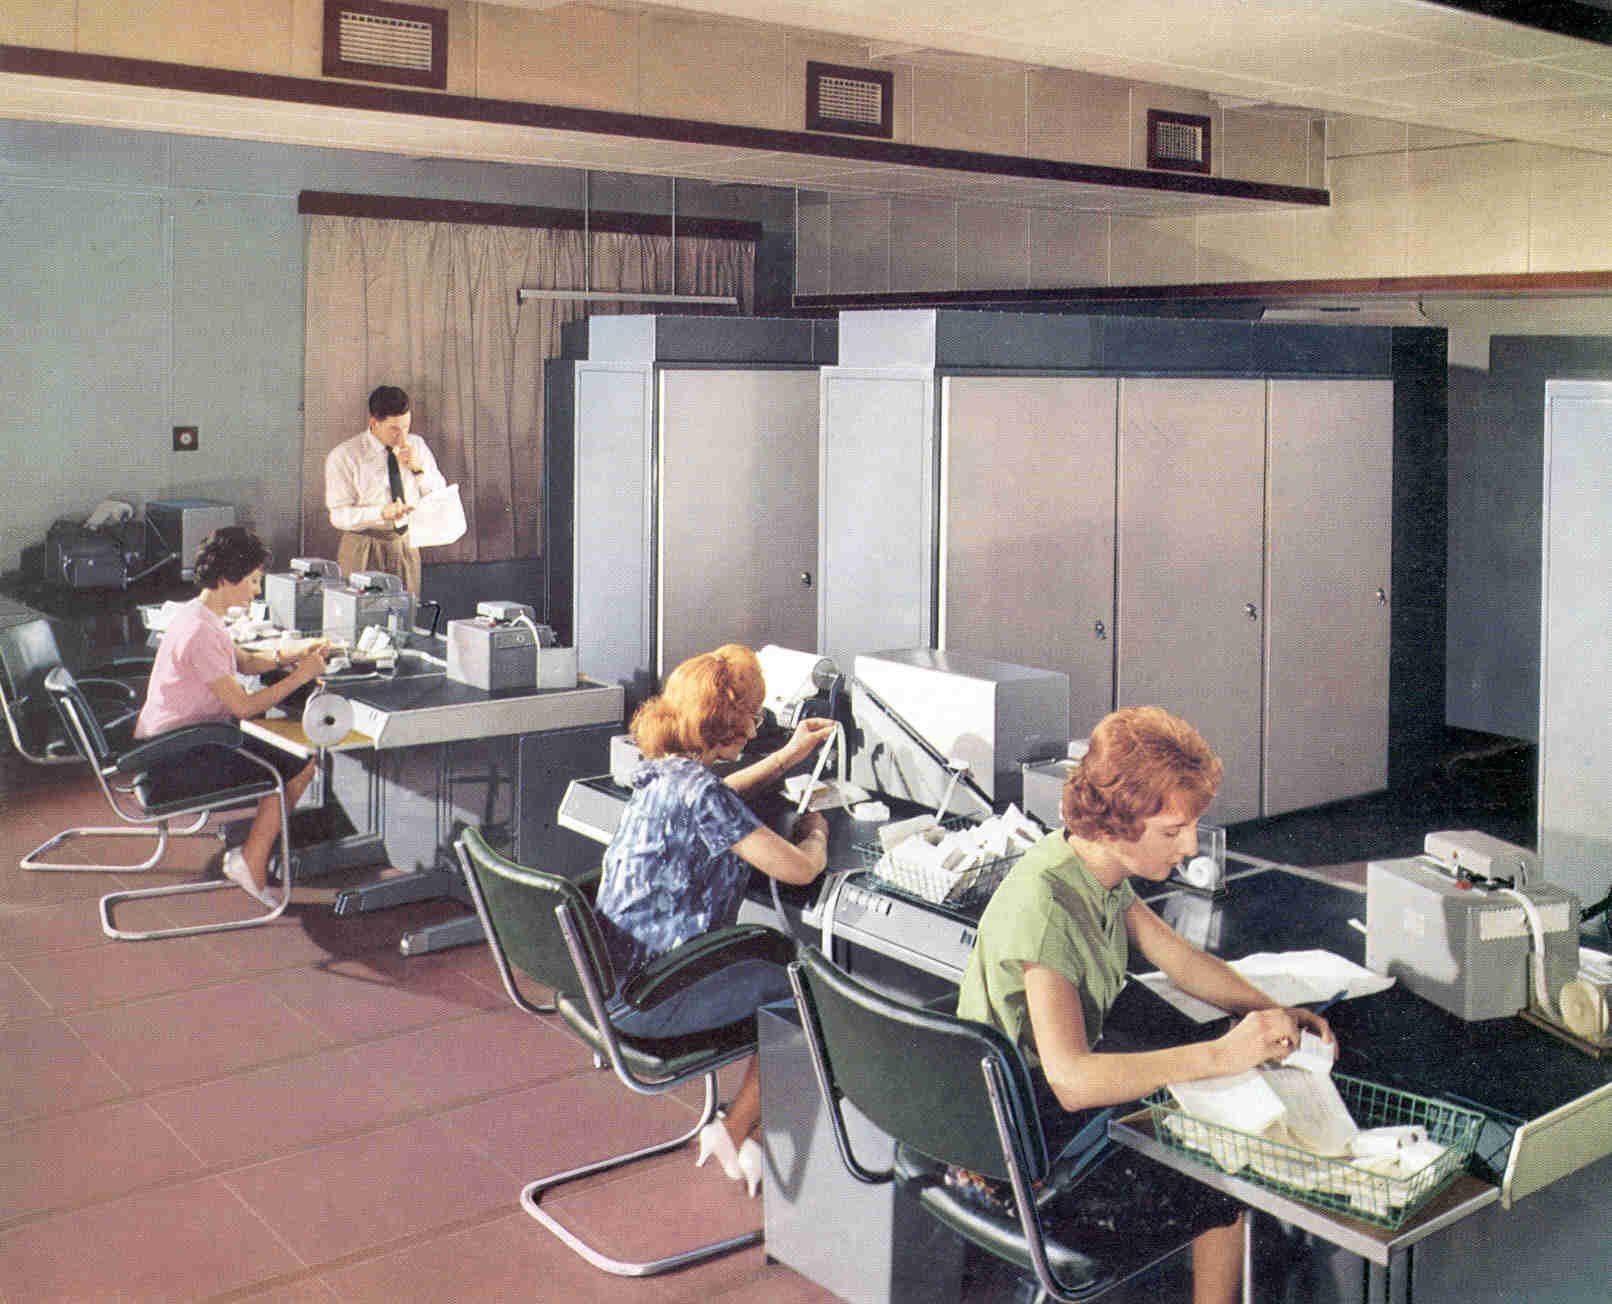
\includegraphics[width=\linewidth]{\currentDir/atlas3}%
}%
\floatSep%
\parbox{0.35\linewidth}{\centering%
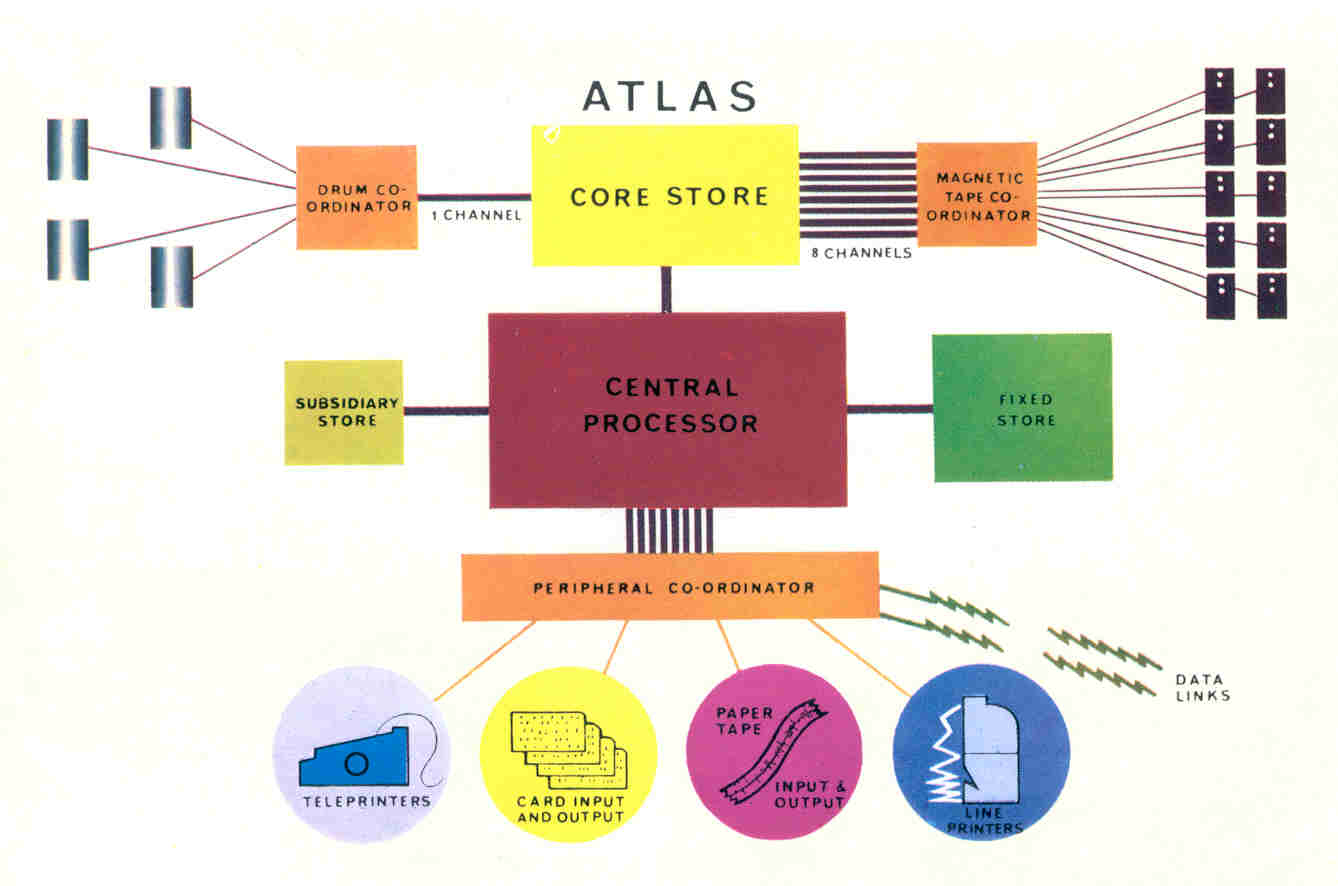
\includegraphics[width=\linewidth,trim={0 10px 0 10px},clip]{\currentDir/atlas1}\\[5pt]%
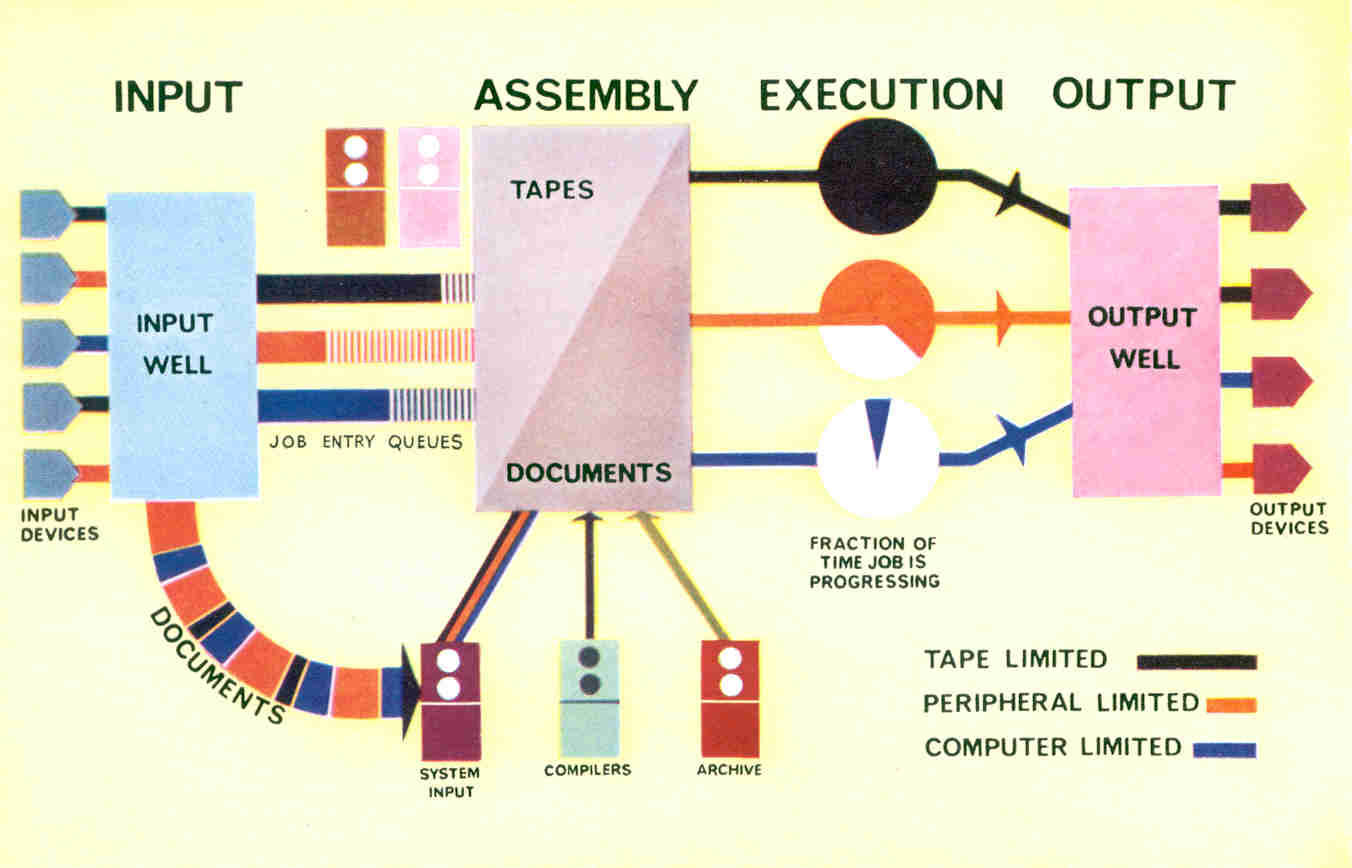
\includegraphics[width=\linewidth,trim={0 10px 0 10px},clip]{\currentDir/atlas2}%
}%
\floatSep%
%
\caption{Images from the \citetitle{M2025CC:FCSA1B1}~\cite{M2025CC:FCSA1B1}. %
\textcopyright~UKRI Science and Technology Facilities Council, available from \url{https://www.chilton-computing.org.uk}.}%
\label{fig:M2025CC:FCSA1B1}%
\end{figure}%

The first file systems for computers appeared in the 1960s.
The Atlas system in the UK had offered a rudimentary file system functionality already in~\citeyear{KPH1961TAS}~\cite{KPH1961TAS,M2025CC:FCSA1B1}, as sketched in~\cref{fig:M2025CC:FCSA1B1}.
The \pgls{OS} \emph{Compatible Time-Sharing System}~(CTSS)~\cite{CMDDCHOK1963TCTSSAPG} at the MIT had a flat filesystem only one or two years later~\cite{OD1963TCCSLABTCDE}.
The hierarchical file system for the \emph{Multics}~\pgls{OS}~\cite{CV1965IAOOTMS}, published in \citeyear{DN1965AGPFSFSS}, already had surprisingly many advanced features that we know from today's file systems: fine-grained access control for data privacy, backup ability, links, and IO~queue management.
File systems are very good for organizing documents and heterogeneous data.
They are not very suitable to main the sort of relational data and to achieve the features that would like \pglspl{db} to have.

The first version of the Integrated Data Store~(IDS) was developed by \citeauthor{B2009TOOTIDSITFDAD} in 1961/62 at General Electric~\cite{B2009TOOTIDSITFDAD,B1965SFRAP}.
IDS offered the first direct access \pgls{db}, holding data in virtual memory.
It may have been the first real \pgls{dbms} and \citeauthor{B2009TOOTIDSITFDAD} won the 1973~A.M.~Turing Award for this work~\cite{H2016HCBITDAFOODW}.
IDS was based on a network model, further advancing data management by structuring complex relationships in data.
The programmer acted as navigator through the data.
The idea to step-by-step navigate through data, updating it if needed, is more complicated and slower compared to the relational approach of today's \pglspl{db}.
IDS and similar systems encode elements of the views of the data as part of the \pgls{db} structure, which make IDS less flexible.
The Database Task Group of the Conference on Data Systems Languages~(CODASYL)~\cite{TF1976CDBMS}, a standardization body for the data processing industry, took over many of \citeauthor{B2009TOOTIDSITFDAD}'s ideas for IDS in the late 1960s.
CODASYL is best known for its creation of the COBOL programming language~\cite{H2016HCBITDAFOODW}.

Only slightly later than IDS, another \pglspl{dbms} that could handle the structured storage of records obeying datatype constraints appeared.
IBM developed the Information Management System~(IMS) for the Apollo space program~\cite{KLBGNLWBS2012ITIYCGTIIMS}.
The system was launched 1965/1967~\cite{BBP2007TBOI}.
IMS is still sold as a product and still exists today.
Like IDS, it was not a \pgls{dbms} for \emph{\pglspl{rdb}}.
Instead, it offered hierarchically structured records.
This system, too, had a set of disadvantages~\cite{KC2024DS:ITD}:
If your data is not structured hierarchically, some records may need to be duplicated.
For example, if we have a database that assigns students to courses, then a student would appear in each of the records of the courses that she attends.
The programming language is also relatively low-level and, for example, the search strategy has to be implemented.
Finally, changes to the logical schema will require us to perform cascading changes in the code accessing them.

Both IDS and IMS offered a strikingly new concept:
The application code and the code for physical data storage and retrieval were separated.
Between them, the Data Language One~(DL/I) was located as interface in IMS.
IDS offered the Data Description Language~(DDL) to define types of logical records and the Data Manipulation Language~(DML) to manipulate and navigate the data.
The \pgls{dbms} controls how the data is stored and loaded.
Application programs can navigate through the data using the much simpler interface languages.
As we briefly mentioned before: \pglspl{dbms} can become arbitrarily complicated pieces of software, and one major part of this is the code to efficiently store and retrieve data.

Just think about it:
All data is eventually mapped/stored to sequential files on a hard disk or other storage medium.
You must be able to add new records and delete old records.
You must also be able to find them.
This alone is not easy to implement, but all of that has to be efficient, so (today) one would probably like to use data structures like hashes, tress, and sorted lists {\dots} all of which are actually located in sequential files.
Before IDS and IMS, this had to be part of your application's code.
Actually, it had to be part of the code of \emph{all} applications that accessed the data, if multiple such applications exist~\cite{BBP2007TBOI}.
Now this is part of IDS and IMS, and the user can ignore this complexity and just use a simple programming language where she can define which record to load, change, delete, or add.%
%
\cquotation{C1970ARMODFLSDB}{Future users of large data banks must be protected from having to know how the data is organized in the machine~(the internal representation).}%
%
In \citeyear{C1970ARMODFLSDB}, the seminal paper \emph{\citetitle{C1970ARMODFLSDB}} by \citeauthor{C1970ARMODFLSDB} appeared, starting with the above quote.
He noticed the shortcomings of the IDS network model, namely that the programmers accessing the data still need a lot of information about how the data is actually represented and organized internally.
Even \citeauthor{B2009TOOTIDSITFDAD} himself mentioned that issues with IDS arose when users did not consider how data is internally sorted~\cite{B2009TOOTIDSITFDAD}.
\Citeauthor{C1970ARMODFLSDB} wanted to protect programmers against such errors.
He models data as a relational view by using tables, that he calls \emph{relations}.
Each column has a type that defines its permitted values.
Each row must be distinct.
One set of columns per table~(usually a single column), the \emph{primary key}, is used to uniquely identify the row.
Rows in one table can references other rows of either the same table or another table.
Therefore, some column(s) of the table~(called \emph{foreign key}) then store the primary key of the row to be reference.
The data in the \pgls{db} is then a collection of tables.
He further describes a set of operations that can work on the tables to extract information, which we will discuss later on.
By the end of the 1970s, over a dozen \pglspl{dbms} had been implemented based on these new concepts~\cite{K1979RDS}.
\Citeauthor{C1970ARMODFLSDB} won the A.M.~Turing Award for his work.

The \emph{semantic} division between the physical storage representation of data and the logical layout and access was a very important step in the development of \pglspl{db}.
This separation also became a \emph{physical} one:
Computer networks as distributed systems began to emerge in the 1960s~\cite{KR2020CNATDA}.
\Citeauthor{B1960OADCACSC} had the idea of routing messages over multiple network switches in~\citeyear{B1960OADCACSC}~\cite{B1964ODCIITDCN,B1964ODCVHAAAC,B1965ABOTDAMBN,B1960OADCACSC,B1962ODCN}.
In \citeyear{K1961IFILCNPTP}, \citeauthor{K1961IFILCNPTP} proposed packet switched networks, where messages are split into multiple packages that each individually travel their corresponding optimal paths~\cite{K1961IFILCNPTP}.
This allows multiple users in a network to share the same data path at the same time.
This idea of packet switching was also independently developed by \citeauthor{B1962ODCN}~\cite{B1962ODCN} and \citeauthor{D1965ROLDPAICN}~\cite{D1965ROLDPAICN,D1965PFTDOANCSFOLDP,D1966PFADCN}.

\begin{figure}%
\centering%
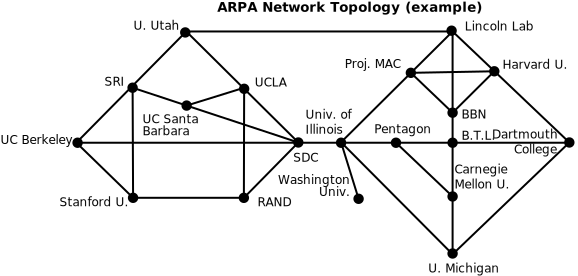
\includegraphics[width=0.8\linewidth]{\currentDir/arpanetRFQ1968}%
\caption{19~node example of the ARPANET structure in the Request for Quotations shipped to vendors in~1968~\cite{K2010AEHOTIHOC}.}%
\label{fig:arpanetRFQ1968}%
\end{figure}%

\Citeauthor{L1963MFMAAOTICN} proposed standardizing computer and networking languages to increase interoperability and to allow researchers to build upon each other's work in~\citeyear{L1963MFMAAOTICN}~\cite{L1963MFMAAOTICN}.
This could be considered as the first description of the idea of the internet.
In 1965/66, the TX\nobreakdashes-2 computer at MIT Lincoln Lab in Massachusetts and the Q\nobreakdashes-32 in Santa Monica, California were connected, forming the first wide-area network~\cite{L1986TAACN}.
In 1967, ARPANET, the precursor of the internet was conceived by the Advanced Research Projects Agency as a network connecting 35~computers at 16~sites in the USA~\cite{L1986TAACN,KR2020CNATDA}.
\Cref{fig:arpanetRFQ1968} shows an 19~node example structure of the ARPANET shipped to vendors in~1968~\cite{K2010AEHOTIHOC}.
In 1969, the first four nodes of the network became operational and in 1972, ARPANET was demonstrated publically~\cite{L1986TAACN,KR2020CNATDA}.

\Citeauthor{CHIRW1974ABECFDBM} proposed putting a \pgls{dbms} on a dedicated back-end computer in~\citeyear{CHIRW1974ABECFDBM}~\cite{CHIRW1974ABECFDBM}.
Applications and users would access the \pgls{dbms} from another computer via a communication link.
The first Ethernet was developed at the Xerox Palo Alto Research Center~(PARC) in 1976 by Metcalfe and Boggs~\cite{CHM1996CLN}, TCP/IP became deployed 1983, and in the 1990s, the internet took off~\cite{KR2020CNATDA}
The term \pglspl{client} was coined in \citeyear{IMS1978SDFFIADFS} by~\citeauthor{IMS1978SDFFIADFS}~\cite{IMS1978SDFFIADFS}.
From now on, the notation of the \pgls{clientServerArchitecture}~\cite{RCKS2019PNP,B1996CSA,OHE1999CSSG,RF2020FOSAAEA,EOEBEB:CSA}, in which most \pglspl{dbms} are implemented today, was formalized.
From then on, the development was unstoppable.

\begin{figure}%
\centering%
\minipage{0.7\linewidth}%
\lstset{style=sql_style,showspaces=False}%
\begin{lstlisting}
SELECT name, student_id FROM table_students
    WHERE date_of_birth >= '2000-01-01';
\end{lstlisting}
\endminipage%
\caption{An example of an \sql\ query.}%
\label{fig:sqlQueryExample}%
\end{figure}%

Another very important step forward for \pglspl{dbms} was the SEQUEL language developed by \citeauthor{CB1974SASEQL} in \citeyear{CB1974SASEQL}~\cite{CB1974SASEQL} as part of the IBM System~R project.
The language was based on \citeauthor{C1970ARMODFLSDB}'s relational algebra, but wrapped it into an easy-to-understand language for data queries.
Two years later, it was extended by more features, such as methods for inserting, deleting, and updating records~\cite{CAEGLMRB1976S2AUATDDMAC}.
In 1977, the SEQUEL name was shortened to \glsreset{SQL}\acrshort{SQL}, an acronym for \acrfull{SQL}~\cite{C20245YOQ}.
An example of an \sql\ query is shown in \cref{fig:sqlQueryExample}.
At the same time where SEQUEL was developed, the Interactive Graphics and Retrieval System~(INGRES) group at the University of Berkeley in California, too, conducted research on \pglspl{db}~\cite{S1986TIPAOARDS}.
The open environment of publishing latest research and collaboration between the researchers contributed significantly to their success.
They jointly received the ACM Software System Award in~1988~\cite{C20245YOQ}.

\begin{figure}%
\centering%
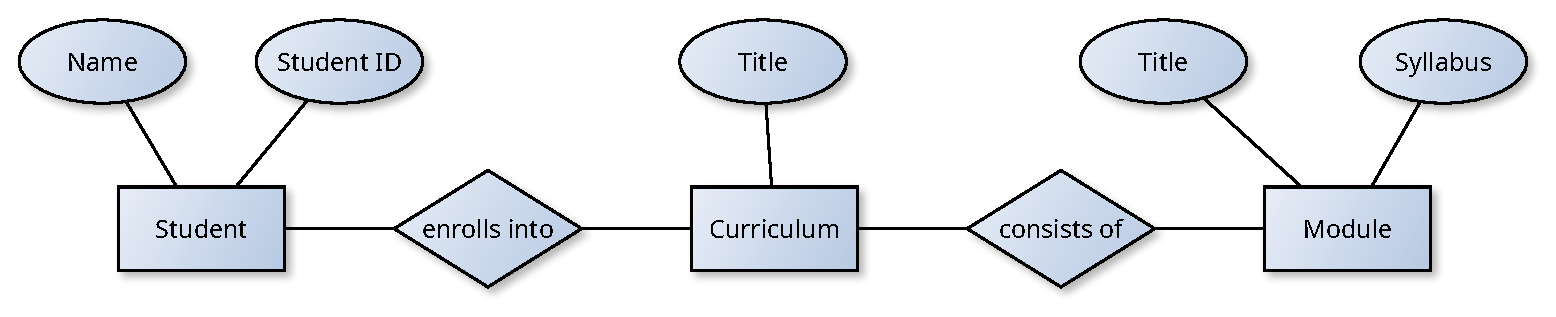
\includegraphics[width=0.9\linewidth]{\currentDir/simpleERDexample}%
\caption{A simple example of an \gls{ERD}.}%
\label{fig:simpleERDexample}%
\end{figure}%

At about the same time where \pgls{SQL} emerged, better abstractions and tools for the design of \pglspl{rdb} began appearing.
\glsreset{ERD}\Pglspl{ERD} like \cref{fig:simpleERDexample} are charts that allow us to model the relationship between different objects in a \db~\cite{KW2012ASHOTEDAIM,C1976TERMTAUVOD}.
They were proposed in~1975 by \citeauthor{C1975TRMTAUVOD}~\cite{C1975TRMTAUVOD} and became part of a US~ANSI standard in the late 1980s~\cite{GK1985ATOOTIRDS,P1992IAX1ASFIRDSI}.
\Citeauthor{C1975TRMTAUVOD}'s work extended the data structure diagrams introduced by \citeauthor{B1969DSD}~\cite{B1969DSD} in \citeyear{B1969DSD} and provided better ways to model attributes and relationships.
\Citeauthor{C1975TRMTAUVOD} was also inspired by his Chinese cultural heritage when developing~\pglspl{ERD}~\cite{C1997ECAED,C2002ERMHEFTALL}:%
%
\cquotation{C1997ECAED}{%
What does the Chinese character construction principles have to do with ER~modeling? %
The answer is: %
both Chinese characters and the ER~model are trying to model the world -- trying to use graphics to represent the entities in the real world. Therefore, there should be some similarities in their constructs.%
}%
%
Oracle \pglspl{db}, the first commercial \pgls{SQL}-based product, was released in 1979~\cite{C20245YOQ} by the company Software Development Laboratories~(SDL), which later renamed itself to Oracle.
It was an immediate success, because it was portable and could run cheaper hardware.
IBM released its \pgls{SQL} \pgls{dbms} DB2 in 1983~\cite{C20245YOQ,HS2013THAGOID}.
\pgls{SQL} became a US~ANSI standard in \citeyear{ANSIX3135} and an international ISO~standard in~\citeyear{ISO90751987}~\cite{ANSIX3135,ISO90751987}.
The standard continues to evolve, with its latest version being released in \citeyear{ISOIEC9707112023E}~\cite{ISOIEC9707112023E}.

In the 1990s, several open source implementations of \pglspl{dbms} became available for free~\cite{C20245YOQ}.
We will discuss them in the next section.%
%
\endhsection%
%
